\documentclass{article}
\usepackage{graphicx} % Required for inserting images
\usepackage{polski}
\input{setup}
\newcommand{\opr}[1]{\mathbf{\hat{#1}}}
\usepackage[margin=2cm]{geometry}
\title{Pakiet KWANT - symulacje transportu elektronowego w~polu magnetycznym}
\author{Marta Wleklińska}
\date{May 2025}

\begin{document}

\maketitle
%%%%%%%%%%%%%%%%%%%%%%%%%%%%%%%%%%%%%%%%%%%%%%%%%%%%%%%%%%%%%%%%%%%%%
\section{Wstęp}
%%%%%%%%%%%%%%%%%%%%%%%%%%%%%%%%%%%%%%%%%%%%%%%%%%%%%%%%%%%%%%%%%%%%%
Obliczanie właściwości transportu kwantowego może być czasochłonne. 
Jednak definiowanie układu oraz metody obliczeniowej może być elastyczne i uniwersalne. 
Aby uniknąć konieczności wielokrotnego pisania kodu od podstaw, opracowano bibliotekę \texttt{Kwant}. Kwant to biblioteka języka \texttt{Python}, która umożliwia łatwe tworzenie, definiowanie oraz obliczanie właściwości transportowych układów kwantowych. 

%%%%%%%%%%%%%%%%%%%%%%%%%%%%%%%%%%%%%%%%%%%%%%%%%%%%%%%%%%%%%%%%%%%%%
\section{Nanodrut}
%%%%%%%%%%%%%%%%%%%%%%%%%%%%%%%%%%%%%%%%%%%%%%%%%%%%%%%%%%%%%%%%%%%%%
Ćwiczenie rozpoczęliśmy od definicji układu nanodrutu.
Będzie on zdyskretyzowany na siatce o długości \texttt{dx}.
Równanie Schr{\"o}dingera po dyskretyzacji przyjmie postać
\begin{equation}
    t(4\psi_{i,j} - \psi_{i-1,j} - \psi_{i+1,j} - \psi_{i,j-1} - \psi_{i,j+1})
    +
    V_{i,j}\psi_{i,j+1}
    =
    E\psi_{i,j},
\end{equation}
gdzie $t = \hbar^2/(2m^*\dd x^2)$.
Pakiet \texttt{Kwant} umożliwia wygodnie obliczyć macierz rozpraszania oraz współczynniki transmisji elektronów przez układ.\\
\\
W celu zbadania wpływu lokalnego potencjału rozpraszającego na transport w nanodrucie, wprowdziliśmy potencjał gaussowski
\begin{equation}
    V(x, y) = V_0\exp\left[\frac{-(x-x_0)^2 - (y-y_0)^2}{\sigma^2}\right],
\end{equation}
zakładając $V_0=50$~meV, $\sigma = 10$~nm.
Konduktancja w takim układzie w funkcji energii została przedstawiona na rysunku~\ref{fig:conductance-nanowire-ex1}.
\begin{figure}[htp!]
    \centering
    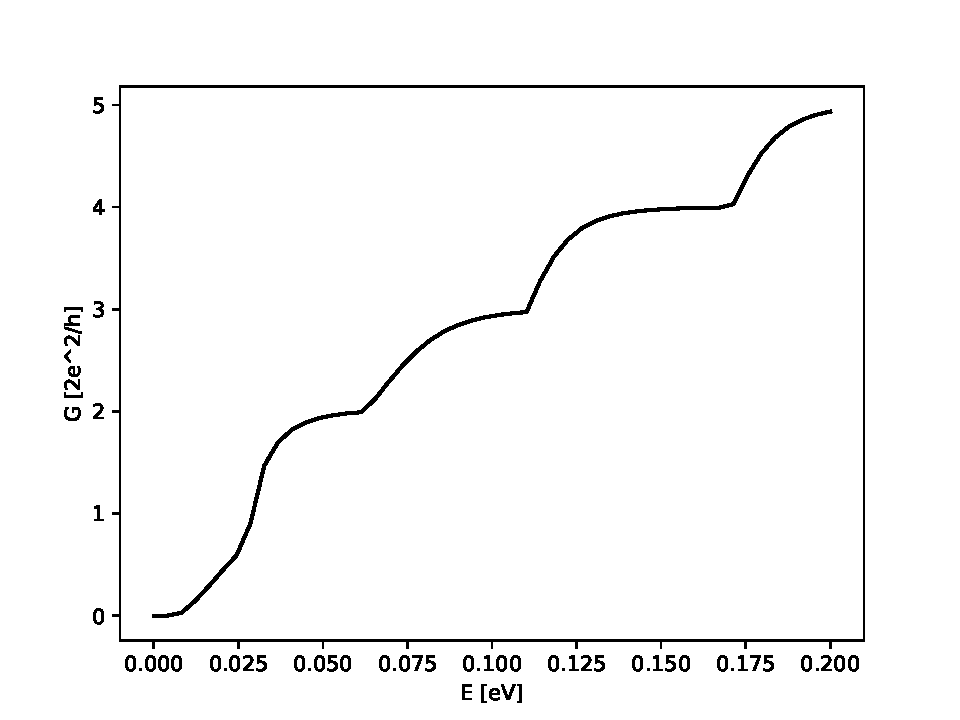
\includegraphics[width=0.65\linewidth]{task1/condutance.pdf}
    \caption{Wykres konduktancji w funkcji energii padającego elektronu dla układu z potencjałem rozpraszania w postaci gaussowskiej zlokalizowanym w środku nanodrutu}
    \label{fig:conductance-nanowire-ex1}
\end{figure}
Można zauważyć typowe dla przewodnictwa kwantowego schodki konduktancji, odpowiadające aktywacji kolejnych modów przewodzenia. Jednakże ich kształt jest wygładzony — efekt ten wynika z rozpraszania na wprowadzonej barierze potencjału. Obecność rozpraszającego centrum prowadzi do częściowej refleksji i modyfikacji funkcji falowych.\\
\\
Następnie rysunek~\ref{fig:task1-waavefunc} zawiera wizualizacje funkcji falowej oraz gęstości prądu dla trzech różnych wartości energii padającego elektronu $E = \{0.02, 0.05, 0.1\}$~eV.
%%%%%%%%%%%%%%%%%%%%%%%%%%%%%%%%%%%%%%%%%%%%%%%%%%%%%%%%%%%%%%%%%%%%%
\begin{figure}[htp!]
    \centering
    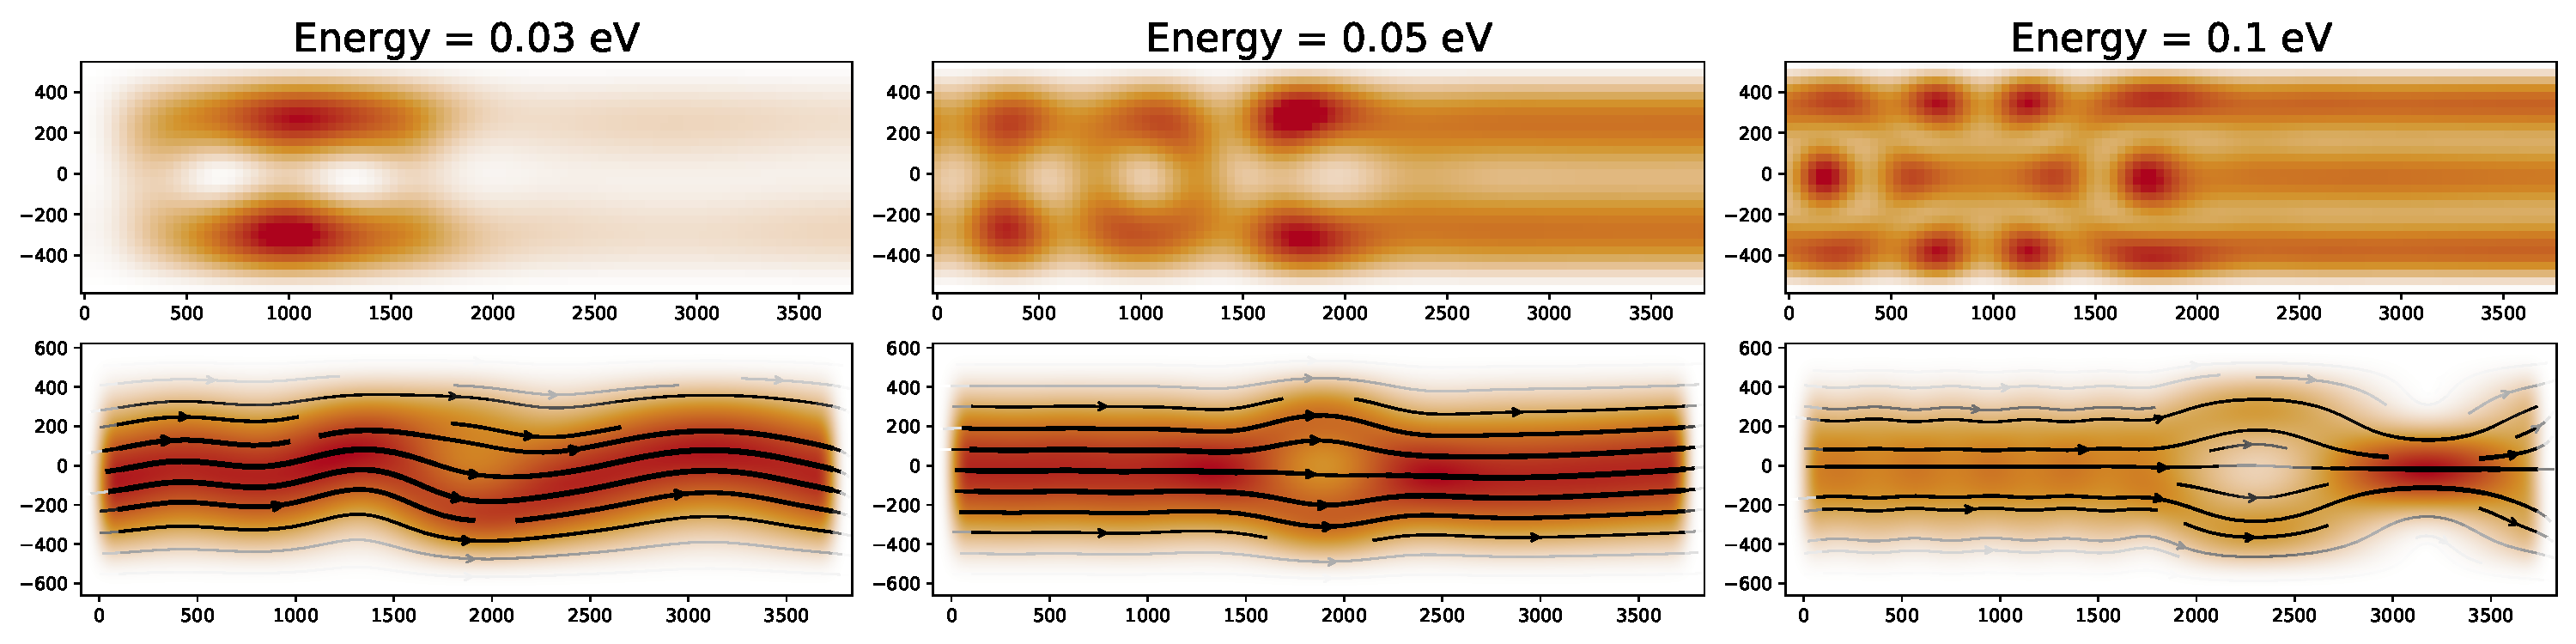
\includegraphics[width=0.9\linewidth]{task1/wavefunctions_currents.pdf}
    \caption{Wykres funkcji falowej oraz gęstości prądu dla układu z potencjałem rozpraszania w postaci gaussowskiej zlokalizowanym w środku nanodrutu dla $E = 0.5$~eV}
    \label{fig:task1-waavefunc}
\end{figure}
 Dla najniższej energii widoczna jest znaczna lokalizacja przed potencjałem, świadcząca o dominującym odbiciu.
 Wraz ze wzrostem energii, funkcje falowe stają się bardziej rozciągnięte przestrzennie, a prąd płynie przez cały układ — wskazując na zwiększoną transmitancję.
 %%%%%%%%%%%%%%%%%%%%%%%%%%%%%%%%%
 \newpage
 \subsection*{Kwantowy efekt Halla}
W kolejnym kroku, chcielibyśmy wprowadzić pole magnetyczne $\mathbf{B} = (0, 0, B_z)$.
W modelu dyskretnym, takim jak stosowany w pakiecie \texttt{kwant}, pole magnetyczne uwzględnia się poprzez odpowiednią fazę dodaną do elementów macierzy Hamiltonianu, zgodnie z regułą Peierlsa.\\
\\
Dla niesymetrycznego cechowania potencjałem wektorowym
\[
\mathbf{A}(x, y) = (-yB_z, 0, 0),
\]
faza Peierlsa pomiędzy punktami $\mathbf{r}_0 = (x_0, y_0)$ oraz $\mathbf{r}_1 = (x_1, y_1)$ dana jest wyrażeniem:
\[
\vartheta = \frac{e}{\hbar} \int_{t(\mathbf{r}_0)}^{t(\mathbf{r}_1)} \dd t\ \mathbf{A}(\mathbf{r}(t))\dv{t}\mathbf{r}(t).
\]
Dokonujemy parametryzacji przez trajektorię prostoliniową między punktami
\[
\mathbf{r}(t) = \mathbf{r}_0 + t(\mathbf{r}_1 - \mathbf{r}_0), \quad t \in [0, 1],
\]
czyli 
\[
x(t) = x_0 + t(x_1 - x_0), \quad y(t) = y_0 + t(y_1 - y_0).
\]
Zatem pochodna zupełna
\[
\dv{\mathbf{r}}{t} = (x_1 - x_0, \ y_1 - y_0).
\]
Mamy teraz wszystkie dane aby wprowadzić do wyrażenia fazę
\[
\vartheta = \frac{e}{\hbar} \int_0^1 \mathbf{A}(\mathbf{r}(t)) \cdot \dv{\mathbf{r}}{t} \, \dd t = \frac{e}{\hbar} \int_0^1 (-B_z y(t))(x_1 - x_0) \, \dd t.
\]
Możemy rozwinąć tę całkę do postaci
\[
\vartheta = -\frac{e B_z}{\hbar} (x_1 - x_0) \int_0^1 (y_0 + t(y_1 - y_0)) \, \dd t
\]
i ją obliczyć
\[
\int_0^1 (y_0 + t(y_1 - y_0)) \, \dd t = y_0 + \frac{1}{2}(y_1 - y_0) = \frac{y_0 + y_1}{2}.
\]
Zatem ostateczna postać fazy Peierlsa wynosi
\[
\vartheta = -\frac{e B_z}{\hbar} (x_1 - x_0) \cdot \frac{y_0 + y_1}{2}.
\]
Tę fazę należy uwzględnić jako czynnik $\ee^{\ii \vartheta}$ w elementach \texttt{hopping}--u.\\
%%%%%%%%%%%%%%%%%%%%%%%%%%%%%%%%%%%%%%%%%%%%%%%%%%%%%%%%%%%%%%%%%%%%%
%%%%%%%%%%%%%%%%%%%%%%%%%%%%%%%%%%%%%%%%%%%%%%%%%%%%%%%%%%%%%%%%%%%%%
\begin{figure}[htp!]
    \centering
\begin{subfigure}{.495\textwidth}
    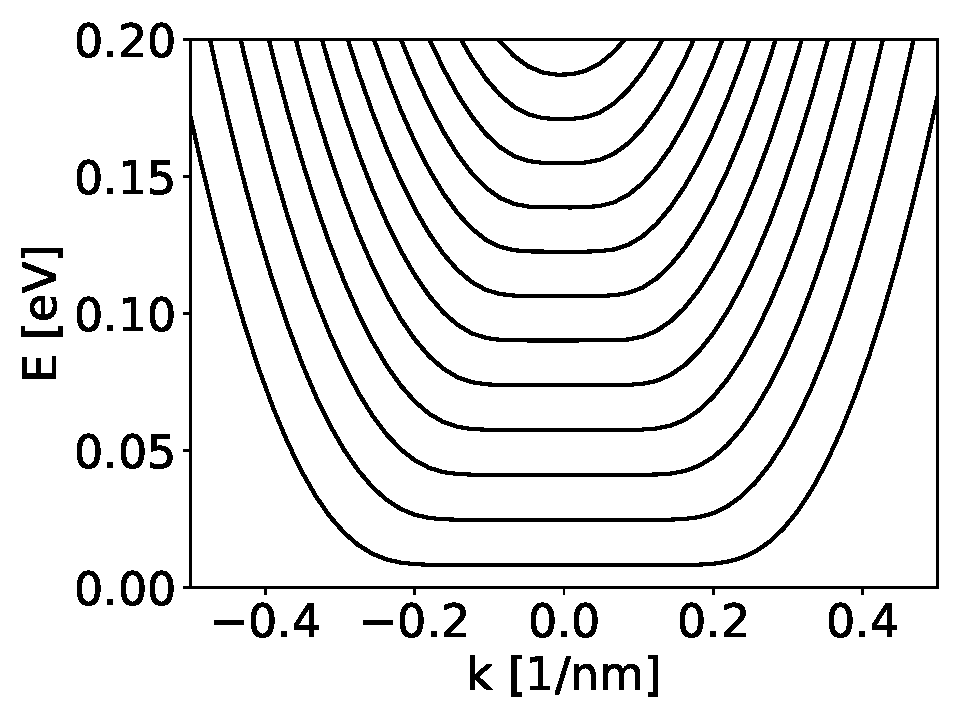
\includegraphics[width=1.0\linewidth]{task2/disp_ex2_B2_100nm.pdf}
    \caption{}
    \label{fig:task2-disp100nm}
\end{subfigure}
\begin{subfigure}{.495\textwidth}
    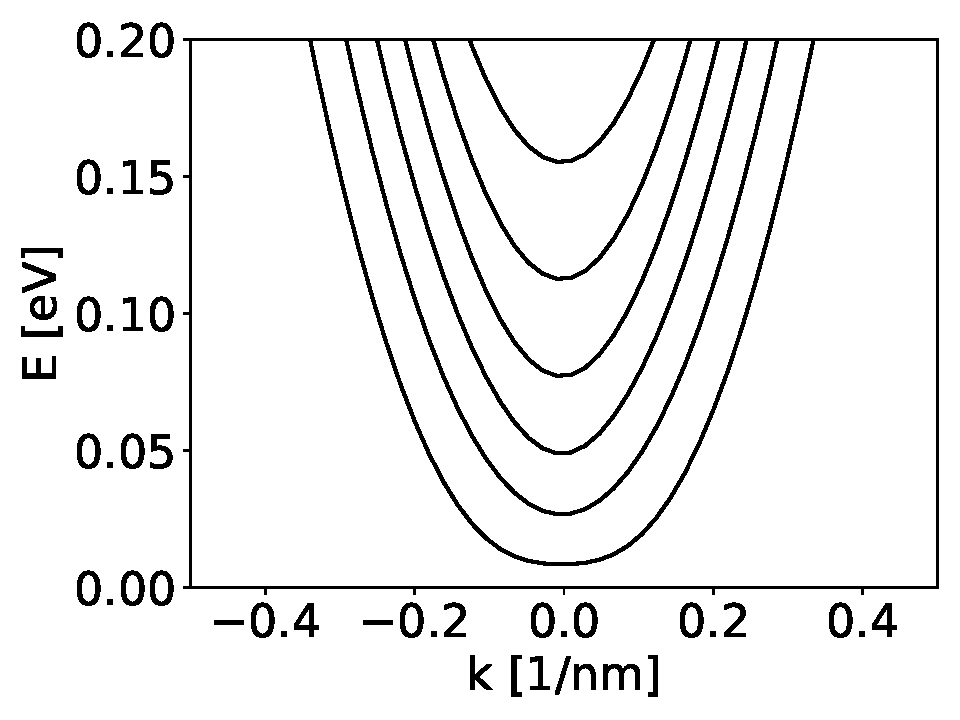
\includegraphics[width=1.0\linewidth]{task2/disp_ex2_B2_40nm.pdf}
    \caption{}
    \label{fig:task2-disp140nm}
\end{subfigure}
\caption{Relacje dyspersji w nanodrucie dla $B_z=2$~T i \textbf{(a)}~$W=200$~nm, \textbf{(b)}~$W=80$~nm}
\label{fig:task2-dispersion}
\end{figure}
\\
Na rysunku~\ref{fig:task2-dispersion} pokazano relacje dyspersji $E(k)$ w lewym kontakcie dla dwóch szerokości nanodrutu: $W = 200$~nm oraz $W = 80$~nm. 
Dla szerszego układu pojawiają się wypłaszczenia przy małych wartościach $k$, charakterystyczne dla stanów Landaua.
Oznacza to, że prąd w tych stanach nie przepływa (grupowa prędkość równa zeru). 
Pojawiające się przerwy energetyczne między stanami sugerują obecność kwantowego efektu Halla — prąd przenoszony jest przez stany brzegowe, które są odporne na rozpraszanie.\\
\\
Na rysunku~\ref{fig:task2-conductance} przedstawiono wykres konduktancji dla tego samego układu.
W porównaniu do wcześniejszego przypadku bez pola magnetycznego, schodki konduktancji są bardziej wyraźne i dobrze zdefiniowane, co świadczy o silniejszej kwantyzacji przewodnictwa.
%%%%%%%%%%%%%%%%%%%%%%%%%%%%%%%%%%%%%%%%%%%%%%%%%%%%%%%%%%%%%%%%%%%%%
\begin{figure}[htp!]
    \centering
    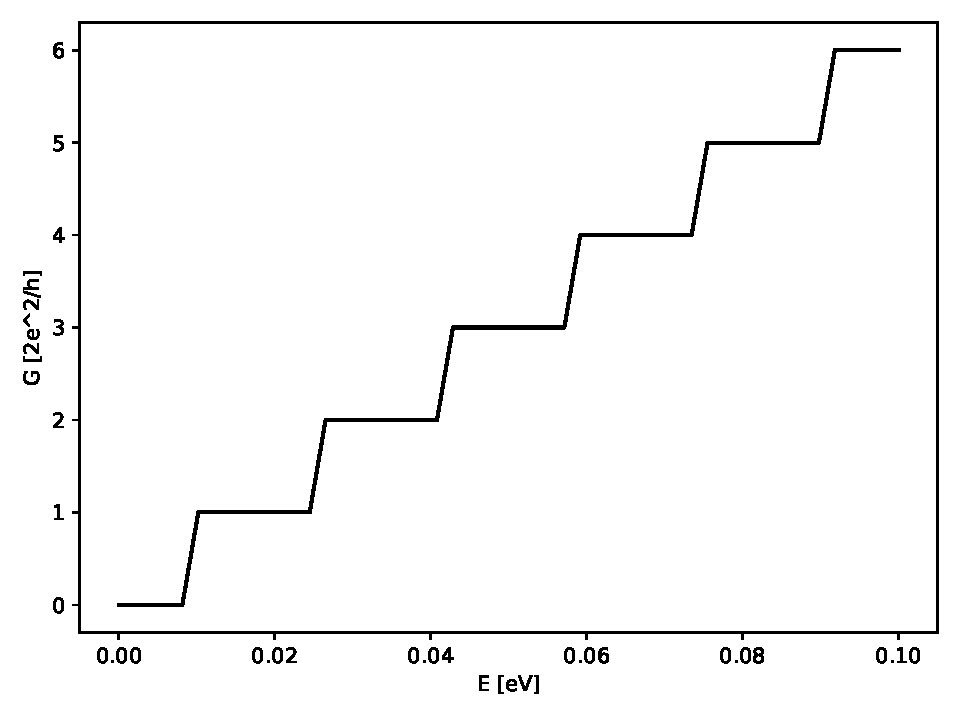
\includegraphics[width=0.65\linewidth]{task2/ex2_condutance.pdf}
    \caption{Wykres konduktancji w funkcji energii padającego elektronu dla $B_z=2$~T i $W = 200$~nm}
    \label{fig:task2-conductance}
\end{figure}
Rysunek~\ref{fig:task2-wavefunction} prezentuje najniższe stany funkcji falowej dla elektronów wpuszczanych z lewego i~prawego kontaktu. 
Obserwujemy ich lokalizację po przeciwnych stronach nanodrutu, co jest efektem działania siły Lorenza i jednoznacznie wskazuje na istnienie stanów brzegowych. \\
%%%%%%%%%%%%%%%%%%%%%%%%%%%%%%%%%%%%%%%%%%%%%%%%%%%%%%%%%%%%%%%%%%%%%
%%%%%%%%%%%%%%%%%%%%%%%%%%%%%%%%%%%%%%%%%%%%%%%%%%%%%%%%%%%%%%%%%%%%%
\begin{figure}[htp!]
    \centering
    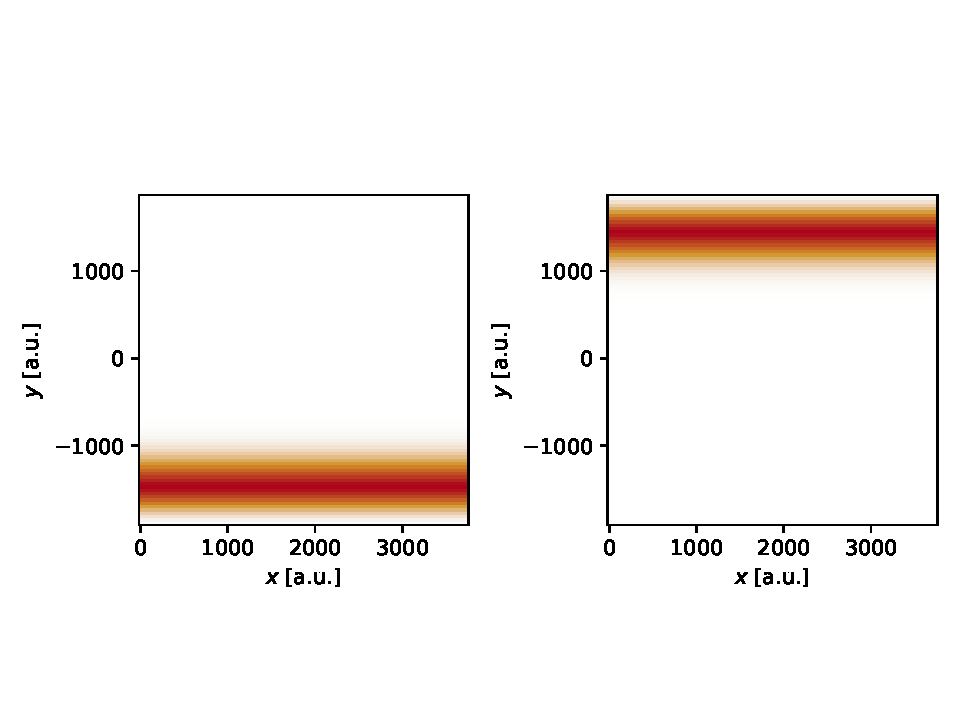
\includegraphics[width=0.65\linewidth]{task2/ex2_wavefunction.pdf}
    \caption{Funkcja falowa najniższego energetycznie stanu dla elektronu puszczonego z lewego i prawego kontaktu.
    Wyniki dla $B_z=2$~T i $W = 80, 200$~nm}
    \label{fig:task2-wavefunction}
\end{figure}
\\
W kolejnej części ponownie dodaliśmy potencjał rozpraszający na górnym brzegu układu.
Ponownie zatem wyznaczyliśmy konduktancję oraz funkcję falową najniższego stanu wstrzykiwanego z lewego kontaktu.
Wykres konduktancji został przedstawiony na rysunku~\ref{fig:task2-conductance-brzeg}, a gęstość prądu oraz funkcja falowa na~\ref{fig:task2/current-wf}.
\begin{figure}[htp!]
    \centering
    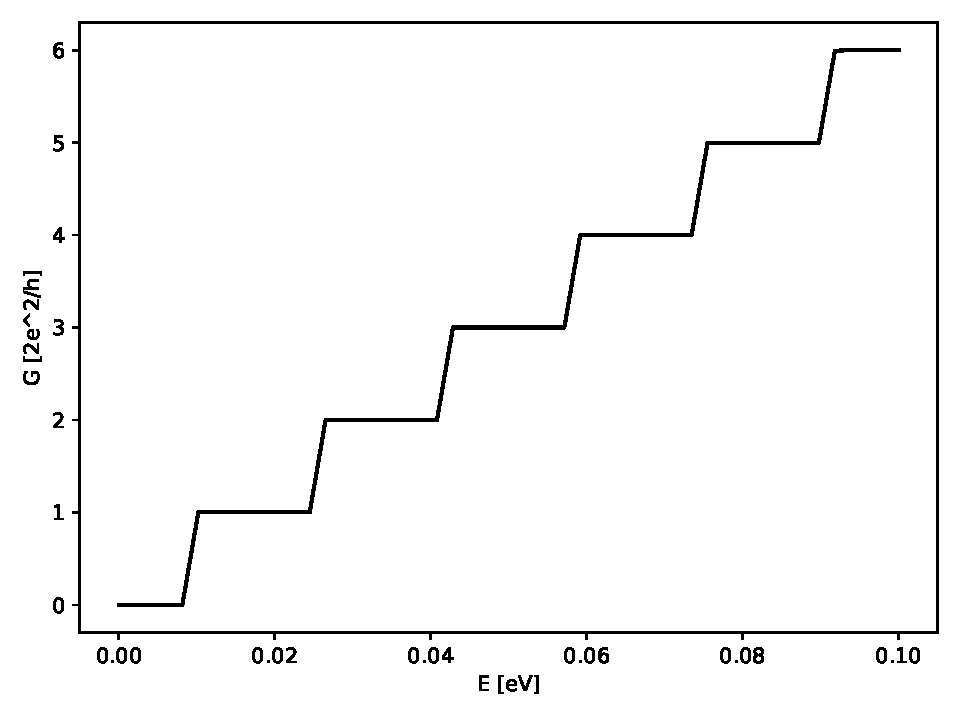
\includegraphics[width=0.6\linewidth]{task2/ex2_condutance_brzeg.pdf}
    \caption{Wykres konduktancji w funkcji energii padającego elektronu przy potencjale rozproszenia na brzegu układu}
    \label{fig:task2-conductance-brzeg}
\end{figure}
\begin{figure}[htp!]
    \centering
    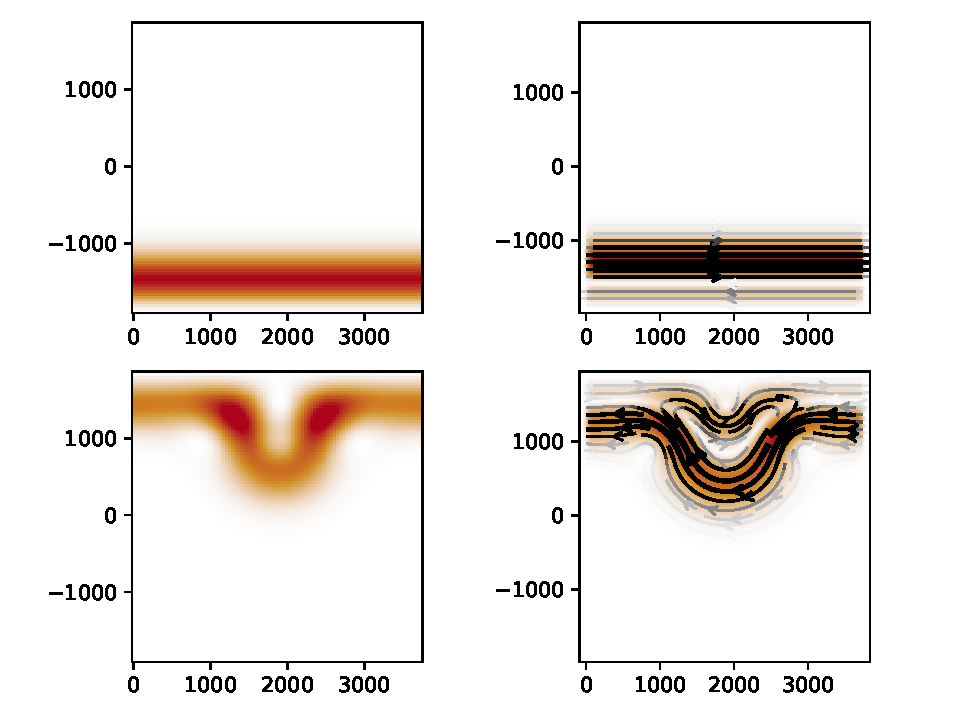
\includegraphics[width=0.65\linewidth]{task2/ex2_wavefunction_brzeg.pdf}
    \caption{Funkcja falowa (wykresy po lewej) i gęstość prądu (po prawej) przy potencjalne rozpraszającym na brzegu układu }
    \label{fig:task2/current-wf}
\end{figure}
Dla wykresów konduktancji nie notujemy dużych zmian przed i po wprowadzeniu potencjału rozpraszania.
Przy mapach funkcji falowej, zauważymy formowanie się przy puszczaniu elektronu z lewego kontaktu pewne \textit{odchylenie} w porównaniu do przypadku bez potencjału.
%%%%%%%%%%%%%%%%%%%%%%%%%%%%%%%%%%%%%%%%%%%%%%%%%%%%%%%%%%%%%%%%%%%%%
%%%%%%%%%%%%%%%%%%%%%%%%%%%%%%%%%%%%%%%%%%%%%%%%%%%%%%%%%%%%%%%%%%%%%

\section{Pierścień kwantowy}
%%%%%%%%%%%%%%%%%%%%%%%%%%%%%%%%%%%%%%%%%%%%%%%%%%%%%%%%%%%%%%%%%%%%%
%%%%%%%%%%%%%%%%%%%%%%%%%%%%%%%%%%%%%%%%%%%%%%%%%%%%%%%%%%%%%%%%%%%%%
Ostatnia część ćwiczenia polegała na symulacji pierścienia kwantowego.
Układ składał się z części kontkatu który został połączony z pierścieniem i wchodził do kontaktu leadu.
Układ został przedstawiony na rysunku~\ref{fig:task3-system}.
\begin{figure}[htp!]
    \centering
    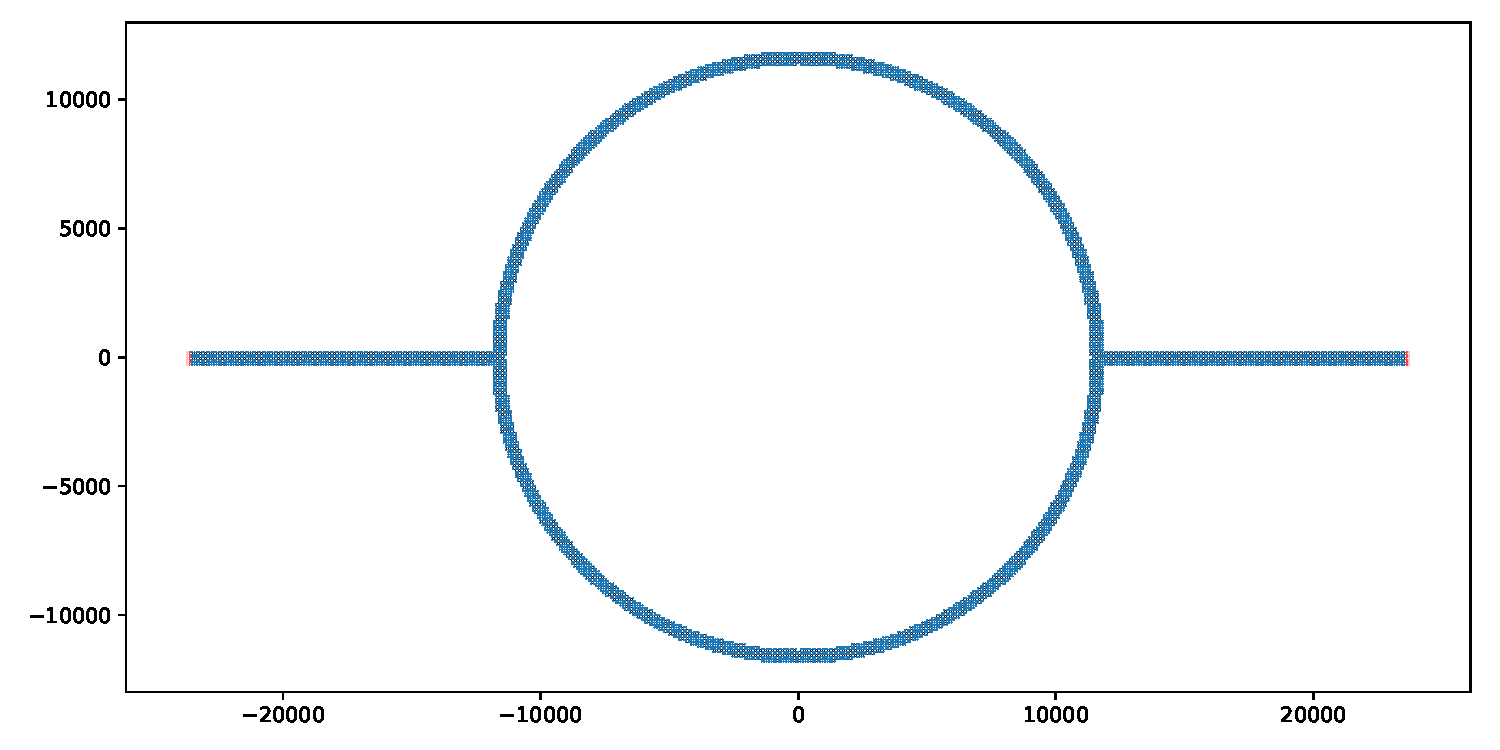
\includegraphics[width=0.5\linewidth]{task3/ex3_ring_system.pdf}
    \caption{Układ pierścienia kwantowego}
    \label{fig:task3-system}
\end{figure}
Ponownie mogliśmy wyznaczyć relację dyspersji, która została zaprezentowana na rysunku~\ref{fig:task3-disperssion}.
\begin{figure}[htp!]
    \centering
    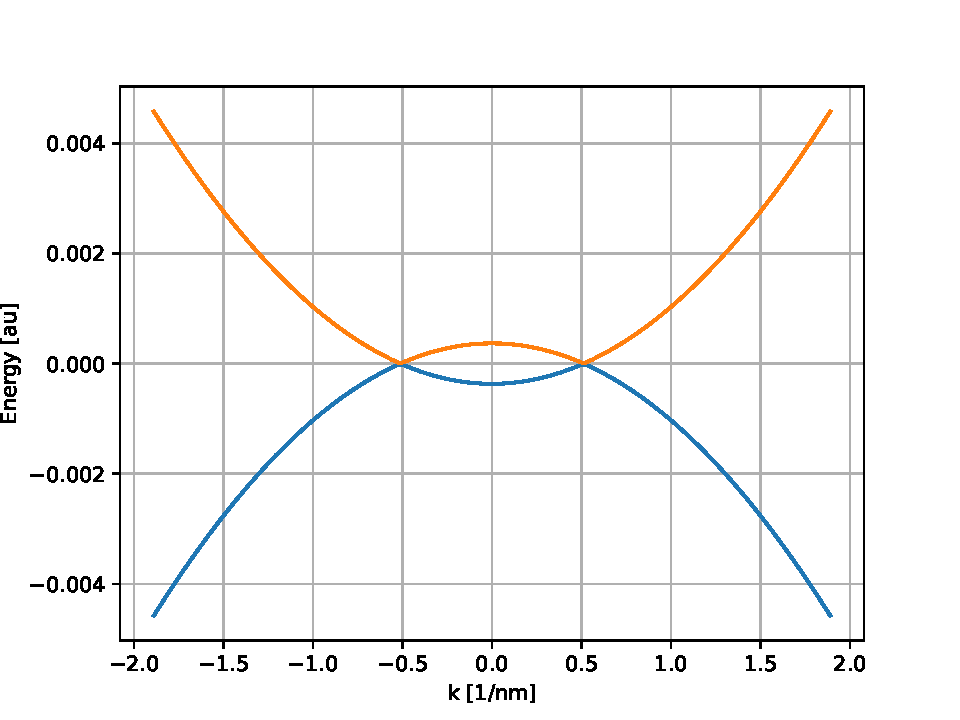
\includegraphics[width=0.5\linewidth]{task3/ex3_dispersion.pdf}
    \caption{Relacja dyspersji dla lewego kanału}
    \label{fig:task3-disperssion}
\end{figure}
Mimo podobnego kształtu do pozostałych relacji z poprzednich części ćwiczenia obserwujemy mniejszą ich gęstość - do wartości $E = 0.2$~eV obserwujemy trzy.
Na rysunku~\ref{fig:task3-conductance} ukazano konduktancję w funkcji pola magnetycznego dla ustalonej energii padającego elektronu ($E = 0.05$~eV). 
\begin{figure}[htp!]
    \centering
    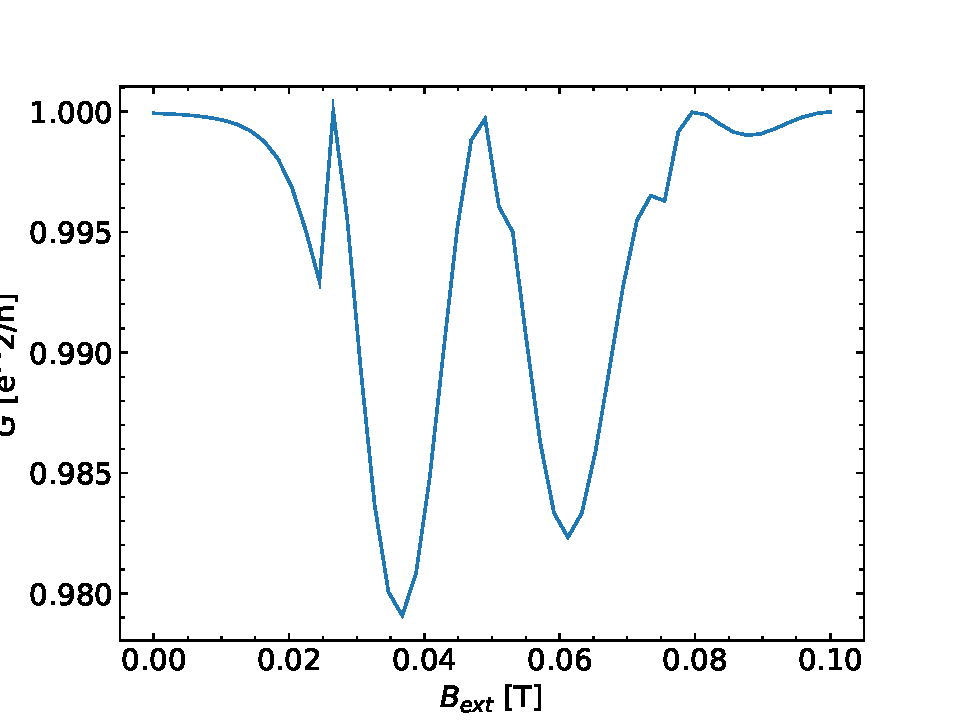
\includegraphics[width=0.56\linewidth]{task3/ex3_conductance.pdf}
    \caption{Konduktancja w funkcji energii przy $E=0.05$~eV}
    \label{fig:task3-conductance}
\end{figure}
Obserwujemy wyraźne oscylacje konduktancji, charakterystyczne dla efektu Aharonova–Bohma. 
Zmiana strumienia magnetycznego przenikającego przez pierścień powoduje interferencję fal elektronowych, prowadzącą do naprzemiennego tłumienia i wzmocnienia transmisji.\\
\\
Odczytując minima i maksima (dla tych pól $B$) mogliśmy wyznaczyć gęstość prądu i funkcje falowe, które zostały przedstawione na rysunku~\ref{fig:task3-current}.
\begin{figure}[htp!]
    \centering
    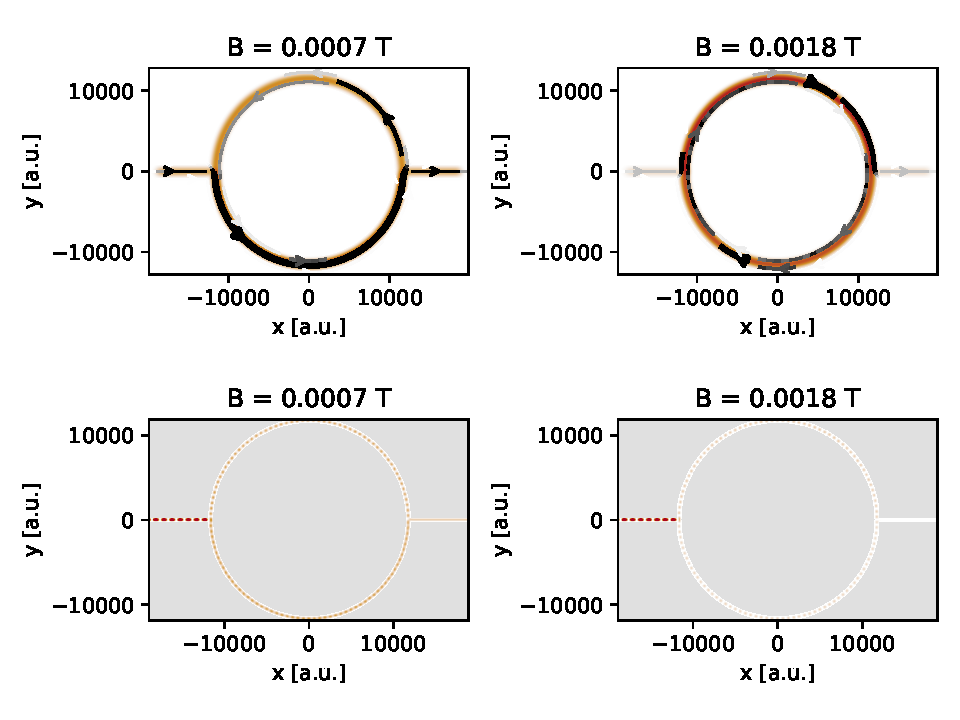
\includegraphics[width=0.7\linewidth]{task3/current_ex3.pdf}
    \caption{Funkcje falowe oraz gęstości prądu przy $B_z=0.7$~mT oraz $B_z = 1.8$~mT}
    \label{fig:task3-current}
\end{figure}
Szczególnie na mapach funkcji falowej możemy zauważyć różnice przy wartości $B_z=1.8$~mT, dla której na zależności konduktancji występowało minimum.
Funkcja falowa jest zlokalizowana w lewym kontakcie.
W przypadku $B_z=0.7$~mT (maksimum konduktancji) występowała ona również w pierścieniu.

\section{Podsumowanie}
Ćwiczenie miało na celu wprowadzić do wykonywania obliczeń w pakiecie \texttt{Kwant}.
Analizowane zostały zależności konduktancji, gęstości prądu sterując parametrami w układach nanodrutu oraz pierścienia kwantowego.
Zaletą tego programu jest dostępne obliczanie parametrów układu, kiedy jedyną trudnością jest definicja układu, co zdecydowanie przyspiesza obliczenia.
\end{document}
